\documentclass[11pt,twoside]{eitExjobb}
%\documentclass[11pt,twoside,final]{eitExjobb}  % Use final for the final version that will be printed
%%%%%%%%%%%%%%%%%%%%%%%%%%%%%%%%%%%%%%%%%%%%%%%%%%%%
%% Other fonts (Palatino as rm font, helvetica as sf font and courier as tt font. All fonts are normally installed with a standard LaTeX distribution.)
% \usepackage{mathpazo} % Also in math mode
% \usepackage[scaled=.95]{helvet}
% \usepackage{courier}
%%%%%%%%%%%%%%%%%%%%%%%%%%%%%
%
\usepackage[utf8]{inputenc}  % Input encoding (this file): 8 bit unicode. Default by most text editors
\usepackage[T1]{fontenc}     % Output encoding (pdf file)
%%%%%%%%%%%%%%%%%%%%%%%%%%%%%
%% Packages used in the example
\usepackage{graphicx}   % Included graphics and some resizable boxes
\usepackage{url}        % nice urls with line breaks 
\usepackage{lipsum}     % nonsense text blocks
\usepackage{booktabs}   % nicer table rules
\usepackage[version=4]{mhchem}   % fancy chemical notation
\usepackage{siunitx}    % better unit notation
\usepackage{fancyref}   % improved labels
\usepackage{parskip}    % better paragraph splitting
\usepackage{subcaption} % easier labeling of subfigures
%%%%%%%%%%%%%%%%%%%%%%%%%%%%%%
\patchcmd{\thebibliography}{\section*{\refname}}{}{}{}
%%%%%%%%%%%%%%%%%%%%%%%%%%%%%%
%%%%%%%%%%%%%%%%%%%%%%%%%%%%%%
\begin{document}
%%% Title page
\Title{Flashlamp Annealing for Improved Ferroelectric Junctions}
\Author{Theodor Blom\\\texttt{nat13tbl@student.lu.se}}
\Supervisor{Mattias Borg}
\CoSupervisor{Rainer Timm}
\Examiner{Mathieu Gisselbrecht}
\Info{12 months, 60 hp}
%% Set by default
% \Date{\today}    %% Today's date
% \Year{\the\year} %% This year shown in copyright
% \Company{Department of Electrical and Information Technology\\Lund University}
%%%%%%
\MakeTitlePage{}  %%% Print title page and copyright page
%%%%%% 
\frontmatter    %%% Page numbering for front pages (small roman)
%%%%% Abstract
\chapter*{Abstract}

%%%%% Abstract
\chapter*{Popular Science Summary}
\subsection*{A New Frontier of Computing}
We all recognize the feeling of panic when your computer crashes and you realize
you forgot to save your progress for the past couple of hours. In this scenario
you wait for the computer to boot again and assess what you have lost. Imagine
instead the computer booting instantly and you find yourself exactly where you
left off. With an emerging technology in computer design this could become the
new reality.

The basic idea behind the fundamental building block of your electronic devices,
known as the transistor, has since its invention in the 1960s been largely
unchanged. The design which proved most successful is known as the
Metal-Oxide-Semiconductor Field Effect Transistor (MOSFET) and is by far the
most common design even to this day due to its cheap manufacturing process and
its ability to be scaled down to ever smaller devices. However, in the last
decade one has started to reach the limits of the MOSFET design, primarily due
to limited scalability, and alternative designs are actively being explored.

A promising design is the Ferroelectric Tunnel Junction (FTJ) which utilizes the
small dimensions of the transistor to its advantage where electrons tunnel
through a thin barrier. This barrier is then manipulated to either allow
electrons though or not, resulting in the characteristic transistor
functionality. In addition to being intrinsically small, the ferroelectric
barrier allows the transistor to be toggleable where the state of the transistor
is maintained even though power is lost. This ability means that electronic
devices utilizing this design does not have to be booted up, as all transistors
are already set to the desired state. Additionally, as power is only consumed as
transistors are being toggled between states, these devices could reduce power
consumption lengthening the battery life across all devices.

However, for this to become the new reality of computers, the FTJ design must be
improved further to prove as an effective alternative to the MOSFET design. One
limiting factor is believed to be the interfaces of the ferroelectric barrier
layer. Utilizing a new technique known as Flash-Lamp Annealing (FLA) the
processing of the ferroelectric barrier layer can be made up to 10 000 times
faster which could significantly improve the interfaces. This as the material
can set much faster resulting in better defined interfaces. If successful, this
could be a crucial step for this new transistor design to become a viable
alternative to MOSFETs and bring in a new frontier of computing.

%% ToC etc
\tableofcontents
\listoffigures
\listoftables
\cleardoublepage{}
%%%%% Page numbering for the main thesis (arabic)
\mainmatter{}
%%%%%%%%%%%%%%%%%%%%%%%%%%%%
\chapter{Introduction}\label{ch:intro}

Mål: Introducera området och ge en överblick.\cite{athle2019development}
    
%%%%%%%%%%%%%%%%%%%%%%%%%%%
\chapter{Semiconductors and Ferroelectrics}\label{ch:semiandferro}

Mål: Klargöra varför III-V (utgå från Si) och FE är intressant. Varför gör vi detta? Vad är applikationern? Få med FTJ här!

\section{Ferroelectricity}

Mål: Basics of FE;\  Polarisation, Domäner och PE-kurvor.

\subsection{\ce{HfZrO2}}

Mål: Redogör för FE-\ce{HfO2} och beskriv hur \ce{Zr} kommer in i bilden. Få med
de olika kristallstrukturerna (faser) här.

\subsection{Capping Using \ce{TiN}}

Mål: Få med att capping suppressar den monocliniska fasen och att det är najs.

\section{III-V Semiconductors}

Mål: Redogör för varför III-V är intressant. Direkt bandgap, lägre DOS --> FTJ

\section{The FTJ Structure and Operation}

Mål: Med FE och III-V förklarat, sammanställ allt i hur en FTJ ser ut och
fungerar med banddiagram och allt.

\subsection{Tunneling and Leakage Mechanics}

Mål: Nämn de olika leakage mechanics i FTJ strukturen. Vi vill helst bara ha
direct tunneling.

\subsection{Thermal Budget and Defects}

Mål: Redogör för vilka typer av defekter vi vill åt och hur de påverkas av
thermal budget. As/In diffusion --> Time dependent --> FLA

%%%%%%%%%%%%%%%%%%%%%%%%%%%
\chapter{Fabrication}\label{ch:fab}

Mål: Redogör för hela processen på LNL.\ 

\section{Processing Methods}

Mål: Redogör för dem mest intressanta/relevanta metoderna. Kanske bara ALD och FLA?\ 

\subsection{ALD}

\subsection{Flashlamp Annealing}

\begin{figure}
    \centering
    \includegraphics[width=.45\linewidth]{example-image}
    \caption{Schematic image of the FLA experimental setup. Should include the
    most important parts such as flashlamps, sample location, preheating
    elements and pyrometer.}\label{fig:fab_FLAsetup}
\end{figure}

\section{Sample Fabrication Process}\label{sec:FabProc}

Mål: Redogör för hela min process.

%%%%%%%%%%%%%%%%%%%%%%%%%%
\chapter{Electrical Characterization}\label{ch:char}

Mål: Redogör för metoderna på E-huset.

\section{PUND and Endurance}\label{sec:PandE}

\section{Capacitance-Voltage}

Frågor att besvara: 
\begin{itemize}
    \item Hur funkar metoderna? 
    \item Vilka defekter ser vi med respektive metod? 
\end{itemize}

%%%%%%%%%%%%%%%%%%%%%%%%%%%
\chapter{Results and Analysis}\label{ch:res}
    %Mål: Presentera serierna i en rimlig ordning och dra slutsatser från varje serie.
    %Tre steg:
    %\begin{enumerate}
        %\item FlashInt och Temperatur
        %\item FlashNum vid olika FlashInt
        %\item Förkristallisering för att minska Tpeak (270C och seedlayer)
    %\end{enumerate}
    %Fokus på frågeställingar!
    %\begin{itemize}
        %\item Utforska möjligheten kring FLA
        %\item Hur bra devices kan vi göra? PUND och Endurance
        %\item Fokus på interface defects genom CV!\  
    %\end{itemize}
\section{Flashlamp Intensity and Film Temperature}
Crystallization of the hafnia films using the flash lamp annealing (FLA)
technique does not immediately reveal the temperature achieved in the films. Due
to the short time frames and the geometry of the FLA setup, one must simulate
the achieved temperature in the film from the structure of the samples and the
flash parameters. Flash duration and preheating temperature were set to
\SI{5}{\milli\second} and \SI{250}{\celsius} respectively in order to be below
the critical crystallization temperature before the FLA
flash~\cite{migita2019phase}. Other simulation parameters are tabulated in
table~\ref{tab:app_simparam} and produce figure~\ref{fig:res_Comsol} showing the
resulting back and front peak temperature for different pulse energies. The figure also
includes pyrometer measurements of the back temperature during annealing
(green). The discrepancies on the order of \SI{20}{\kelvin} between simulated
back peak temperature (black) and the measured values are attributed to a likely
lower reflectivity of the \ce{TiN} capping layer compared to the ideal values of
the simulation. Therefore, the model is deemed to be in reasonable agreement
with the experimental data and gives an estimate of the achieved surface peak temperature.

\begin{figure}[htbp]
    \centering
    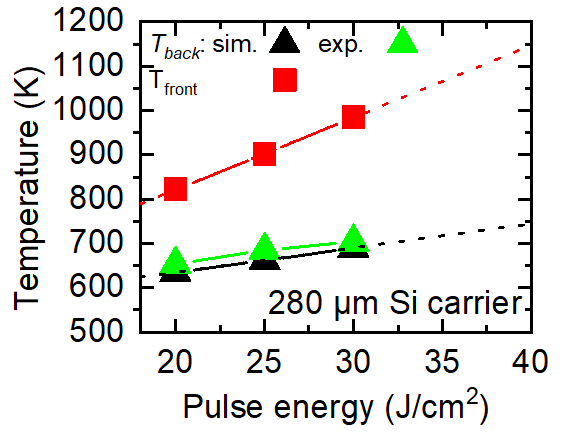
\includegraphics[width=.41\linewidth]{fig/COMSOLFlashInt.png}
    \caption{Simulated back and front peak temperatures of our samples using the
    simulation parameters tabulated in~\ref{tab:app_simparam}. Pyrometer
    measurements of the back temperature measured during annealing (green) confirm
    the accuracy of these simulations.}\label{fig:res_Comsol}
\end{figure}

Figure~\ref{fig:res_Comsol} reveal a linear relationship between the pulse
energy ($E_{pulse}$) and the peak HZO film temperature ($T_{peak}$) for our
sample and FLA parameters (eq~\ref{eq:app_filmtemp}). This gives a more
convenient reference going forward using the achieved film temperature rather
than the pulse energy when describing different samples. The usually reported
crystallization temperature required to form the ferroelectric orthorhombic
phase of HZO is in the range of 670~-
\SI{870}{\kelvin}~\cite{muller2012ferroelectricity, athle2022improved}.
The simulated peak surface temperatures in the 20~-
\SI{30}{\joule\per\square\centi\meter} pulse energy range are significantly
above this critical temperature and should therefore yield a sufficiently high
peak temperature to achieve ferroelectric properties in the HZO.\@

\section{Sample Specifications and Characterization}
As a reference point, samples were processed using rapid thermal processing
(RTP) as the annealing method in parallell to the FLA samples. These samples
proves as a point of comparison for the characterization of the FLA samples
throughout the work. The RTP samples were annealed at a temperature of
\SI{870}{\kelvin} for 30 seconds. The electrical characterization of these
samples, as described in Chapter~\ref{ch:char} the remnant polarization ($P_r$),
coercive field ($E_c$), endurance and defect density ($D_d$) were measured and
tabulated in table~\ref{tab:RTPref}.

\begin{table}[htbp]
    \centering
    \caption{Electrical characteristics for the RTP reference samples.}\label{tab:RTPref}
    \begin{tabular}{rlrl}
        \toprule
        \multicolumn{4}{c}{PUND and Endurance}\\\midrule
        Remnant Polarization & $P_r$ & $29.03 \pm 0.21$ & \si{\micro\coulomb/\centi\meter^2}\\
        Coercive Field & $E_c$ & $1.23 \pm 0.18$ & \si{\mega\volt/\centi\meter}\\
        Endurance & & $23 \pm 11$ & $10^3$ cycles\\
        Defect Density & $D_d$ & $10.0 \pm 1.0$ &
        $10^{12}$ \si{\per\square\centi\meter}
        \\\bottomrule
    \end{tabular}
\end{table}

The processing of the FLA samples are outlined in Section~\ref{sec:FabProc}. For
the first FLA series, hereby denoted sample series 1, the flash intensity was
varied between 15-\SI{32.5}{\joule/\centi\meter^2} to reach different peak
temperatures in the film. The film deposition and annealing conditions for these
samples are summarized in table~\ref{tab:res_IntC}.

\begin{table}[htbp]
    \centering
    \caption{Selected processing conditions for sample series 1.}\label{tab:res_IntC}
    \begin{tabular}{rlccccc}
        \toprule
        \multicolumn{2}{l}{Sample Number} & 1 & 2 & 3 & 4 & 5 \\\midrule
        \multicolumn{1}{c}{HZO} & & & & & & \\
        Growth Temperature & [\si{\celsius}] & 200 & 200 & 200 & 200 & 200 \\
        Film Thickness & [\si{\nano\meter}] & 10 & 10 & 10 & 10 & 10 \\\midrule
        \multicolumn{1}{c}{FLA} & & & & & & \\
        Preheat Temperature & [\si{\celsius}] & 250 & 250 & 250 & 250 & 250 \\
        Flash Intensity & [\si{\joule/\centi\meter^2}] & \textbf{15} & \textbf{20} & \textbf{25} & \textbf{30} & \textbf{32.5} \\
        Number of Flashes & & 1 & 1 & 1 & 1 & 1 \\\bottomrule
    \end{tabular}
\end{table}

Resulting electrical characterization from sample series 1 are shown in
figure~\ref{fig:res_IntC}. Samples annealed with an intensity less than
\SI{25}{\joule/\centi\meter^2} did not show any ferroelectric behaviour and are
hence omitted from some of the figures. As shown in
figure~\ref{fig:res_IntC}a and b the PUND characteristics show
ferroelectric behaviour with a strong dependance on peak film temperature.
However, for higher peak temperatures these characteristics decline to both
weaker polarization response and higher coercive fields which is undesireable.
The peak PUND performance at \SI{30}{\joule/\centi\meter^2} does not reach the
characteristics of the RTP references outlined in table~\ref{tab:RTPref} which
shows that the energy deposited during the annealing process is not enough to
crystalize the entire HZO film while not inducing other effects to reduce the
ferroelectric response.

Although reduced PUND characteristics were found for these samples,
figure~\ref{fig:res_IntCEndu} show an increased endurance for the flash
annealed samples compared to the RTP reference.

\begin{figure}[htbp]
    \centering
    \begin{subfigure}{.4\linewidth}
        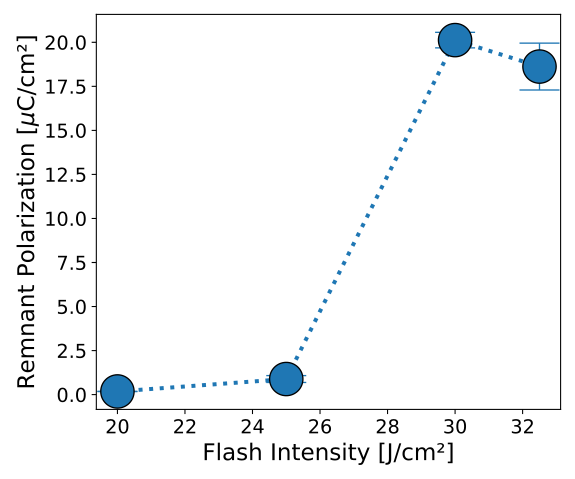
\includegraphics[width=\linewidth]{fig/FlashIntC_PrTrends.png}
        \caption{}\label{fig:res_IntCPr}
    \end{subfigure}
    \begin{subfigure}{.4\linewidth}
        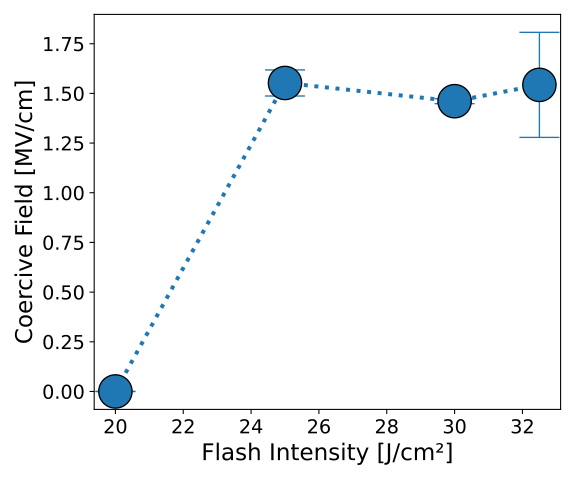
\includegraphics[width=\linewidth]{fig/FlashIntC_EcTrends.png}
        \caption{}\label{fig:res_IntCEc}
    \end{subfigure}
    \begin{subfigure}{.4\linewidth}
        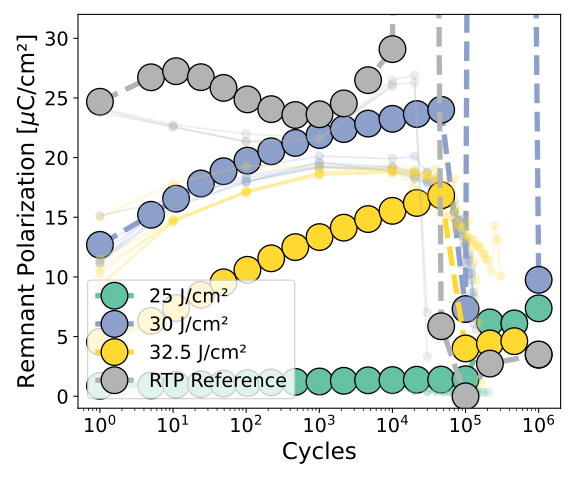
\includegraphics[width=\linewidth]{fig/FlashIntC_EnduTrends.png}
        \caption{}\label{fig:res_IntCEndu}
    \end{subfigure}
    \begin{subfigure}{.4\linewidth}
        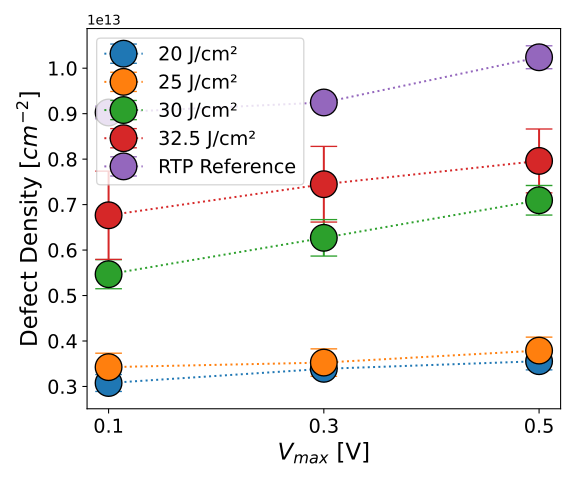
\includegraphics[width=\linewidth]{fig/FlashIntC_DDTrends.png}
        \caption{}\label{fig:res_IntCDD}
    \end{subfigure}
    \caption{Figure showing all measured data from an intensity-varied batch.
    Low-doped subtrate, 200C ALD, HZO 1:1, 250C preheat, 5ms flash. RTP
    reference is included for Endurance and Defect Density.}\label{fig:res_IntC}
\end{figure}

%\begin{figure}[htbp]
    %\centering
    %(a)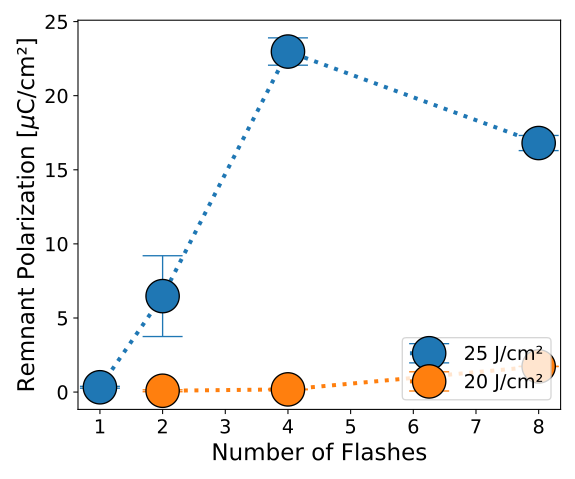
\includegraphics[width=.45\textwidth]{../Fig/FlashNumA+C_PrTrends.png}
    %(b)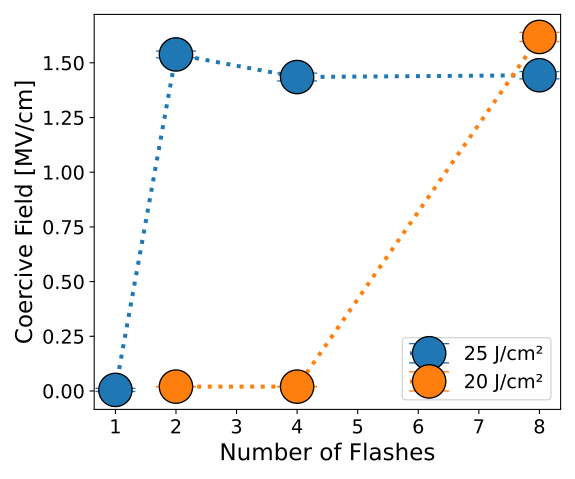
\includegraphics[width=.45\textwidth]{../Fig/FlashNumA+C_EcTrends.png}
    %\caption{Figure showing Pr and Ec trends from flashnumber-varied batches. Low-doped subtrate, 200C ALD, HZO 1:1, 250C preheat, 5ms flash at $\SI{25}{\joule/\centi\meter^2}$ and \SI{20}{\joule/\centi\meter^2}.}\label{fig:res_FlashNumAC_PrEc}
%\end{figure}

%\begin{figure}[htbp]
    %\centering
    %(a)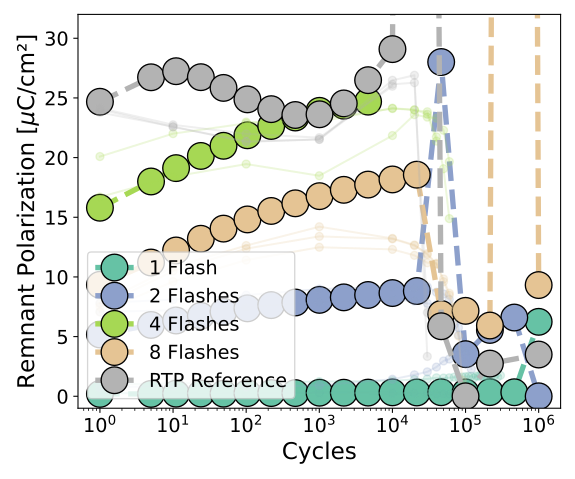
\includegraphics[width=.45\textwidth]{../Fig/FlashNumA_EnduTrends.png}
    %(b)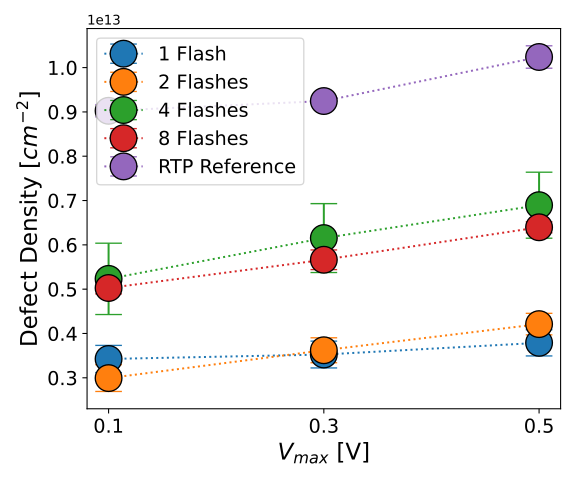
\includegraphics[width=.45\textwidth]{../Fig/FlashNumA_DDTrends.png}
    %(c)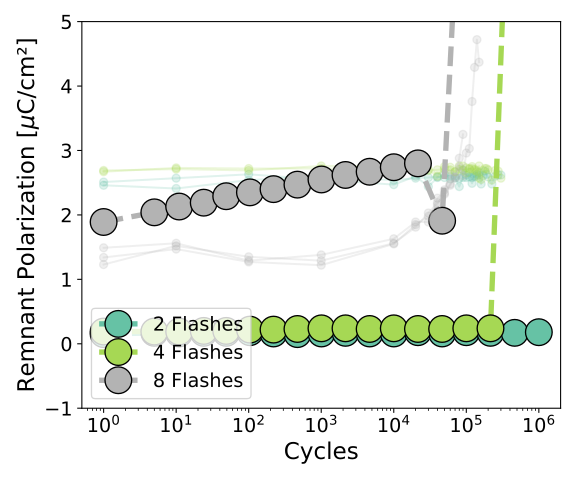
\includegraphics[width=.45\textwidth]{../Fig/FlashNumC_EnduTrends.png}
    %(d)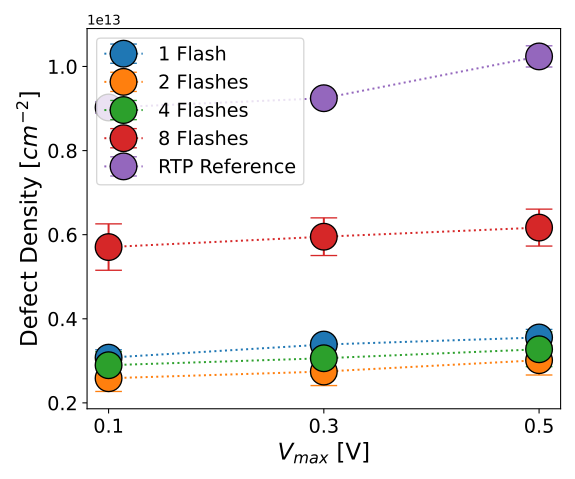
\includegraphics[width=.45\textwidth]{../Fig/FlashNumC_DDTrends.png}
    %\caption{Figure showing Endurance and Defect Density from flashnumber-varied batches. Low-doped subtrate, 200C ALD, HZO 1:1, 250C preheat, 5ms flash at $\SI{20}{\joule/\centi\meter^2}$. RTP reference is included.}\label{fig:res_FlashNumAC_EnduDD}
%\end{figure}

%\begin{figure}[htbp]
    %\centering
    %(a)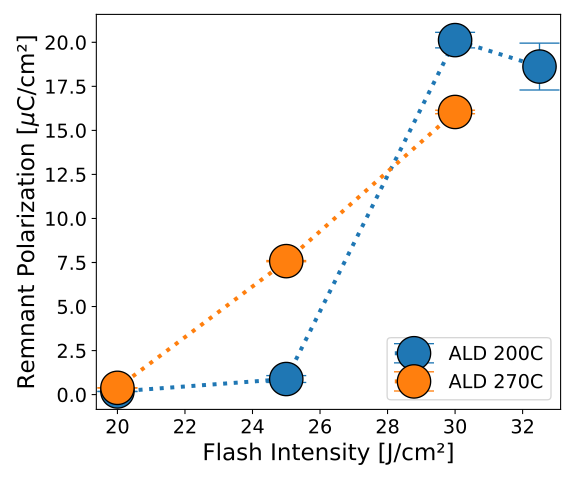
\includegraphics[width=.45\textwidth]{../Fig/FlashIntC+E_PrTrends.png}
    %(b)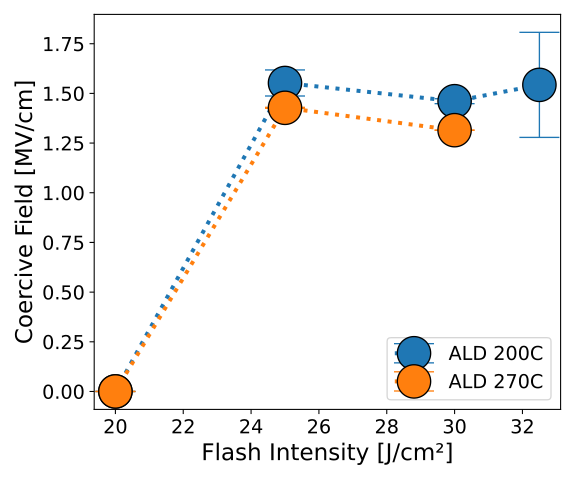
\includegraphics[width=.45\textwidth]{../Fig/FlashIntC+E_EcTrends.png}
    %(c)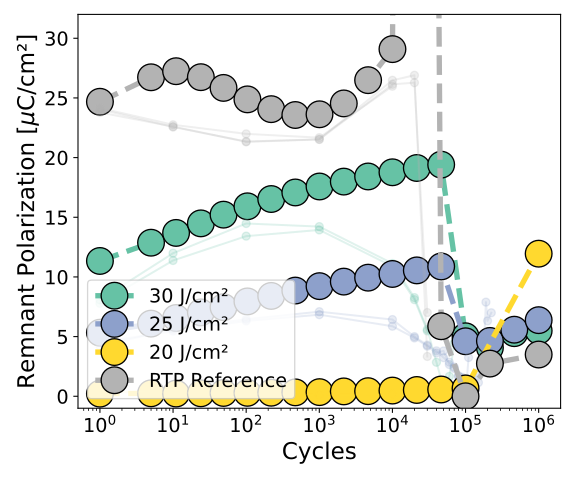
\includegraphics[width=.45\textwidth]{../Fig/FlashIntE_EnduTrends.png}
    %(d)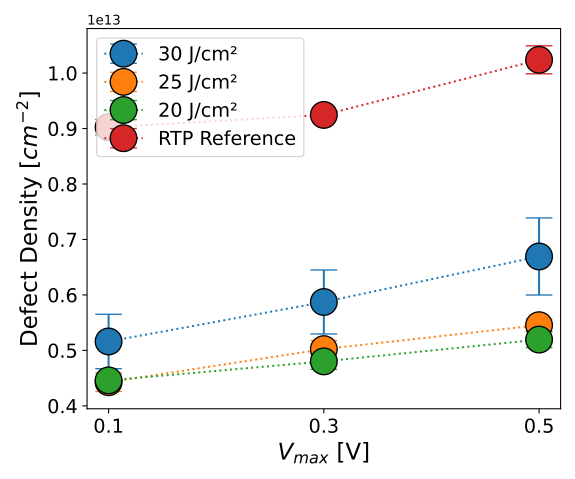
\includegraphics[width=.45\textwidth]{../Fig/FlashIntE_DDTrends.png}
    %\caption{Figure showing all measured data from an intensity-varied batch. Low-doped subtrate, 270C ALD, HZO 1:1, 250C preheat, 5ms flash. RTP reference is included for Endurance and Defect Density.}\label{fig:res_FlashIntE}
%\end{figure}

%\begin{figure}[htbp]
    %\centering
    %(a)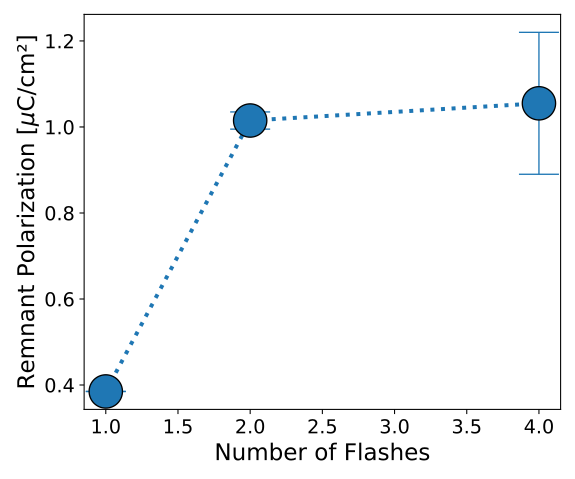
\includegraphics[width=.45\textwidth]{../Fig/FlashNumD_PrTrends.png}
    %(b)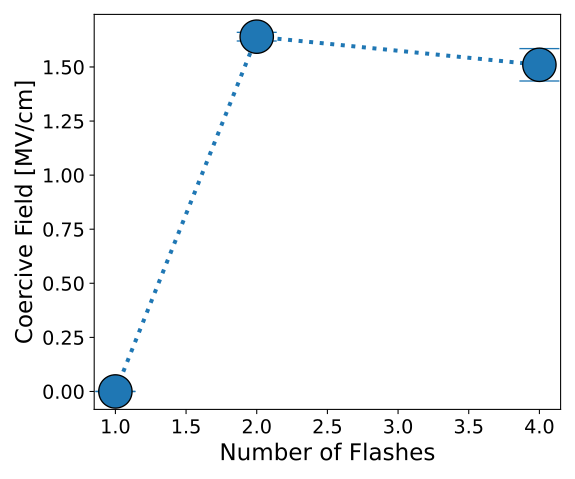
\includegraphics[width=.45\textwidth]{../Fig/FlashNumD_EcTrends.png}
    %(c)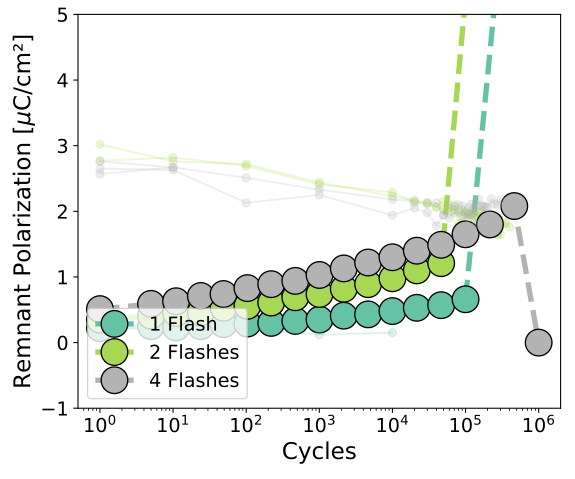
\includegraphics[width=.45\textwidth]{../Fig/FlashNumD_EnduTrends.png}
    %(d)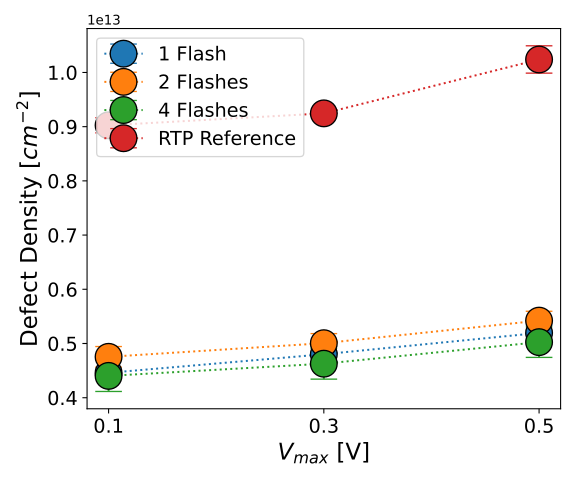
\includegraphics[width=.45\textwidth]{../Fig/FlashNumD_DDTrends.png}
    %\caption{Figure showing all measured data from a flashnumber-varied batch. Low-doped subtrate, 270C ALD, HZO 1:1, 250C preheat, 5ms flash.}\label{fig:res_FlashNumD}
%\end{figure}

%%%%%%%%%%%%%%%%%%%%%%%%%%
\chapter{Conclussion}\label{chap:conc}

Mål: Wrap it up. Lägg fram de främsta resultaten/ideerna och ge tips på hur man
kan undersöka vidare.

%%%%%%%%%%%%%%%%%%%%%%%%%%%%%%%%%%%%%%%
%% References
\bibliography{Exjobbreport.bib}
\bibliographystyle{ieeetr}


%%%%%%%%%%%%%%%%%%
\appendix
%%%%%%%%%%%%%%%%%%%
\chapter{Extra material}
\begin{table}[htbp]
    \centering
    \caption{Relevant simulation parameters used in COMSOL to achieve
    figure~\ref{fig:res_Comsol}. The \ce{InAs/HZO/TiN} is part of the sample
while \ce{Si} is a carrier wafer part of the FLA experimental setup.}\label{tab:app_simparam}
    \begin{tabular}{crcc}
        \toprule
        Layer & Thickness & Doping & Reflectivity \\\midrule
        \ce{TiN} & \SI{10}{\nano\meter} &~- & 0.41 \\ 
        \ce{HZO} & \SI{10}{\nano\meter} & 1:1 (\ce{Hf/Zr}) &~- \\ 
        \ce{InAs} & \SI{280}{\micro\meter} & \SI{1e16}{\per\centi\meter\tothe{3}} &~- \\ 
        \ce{Si} & \SI{280}{\micro\meter} &~- &~- \\\bottomrule
    \end{tabular}
\end{table}

\begin{equation}\label{eq:app_filmtemp}
    T_{peak} [\si{\kelvin}] = 495.5 + 16.3 \cdot E_{pulse} [\si{\joule\per\square\centi\meter}]
\end{equation}

\end{document}
